\documentclass{beamer}
\usepackage[utf8]{inputenc}

\usetheme{Madrid}
\usecolortheme{default}
\usepackage{amsmath,amssymb,amsfonts,amsthm}
\usepackage{txfonts}
\usepackage{tkz-euclide}
\usepackage{listings}
\usepackage{adjustbox}
\usepackage{array}
\usepackage{tabularx}
\usepackage{gvv}
\usepackage{lmodern}
\usepackage{circuitikz}
\usepackage{tikz}
\usepackage{graphicx}
\usepackage{mathtools}
\setbeamertemplate{page number in head/foot}[totalframenumber]

\usepackage{tcolorbox}
\tcbuselibrary{minted,breakable,xparse,skins}



\definecolor{bg}{gray}{0.95}
\DeclareTCBListing{mintedbox}{O{}m!O{}}{%
  breakable=true,
  listing engine=minted,
  listing only,
  minted language=#2,
  minted style=default,
  minted options={%
    linenos,
    gobble=0,
    breaklines=true,
    breakafter=,,
    fontsize=\small,
    numbersep=8pt,
    #1},
  boxsep=0pt,
  left skip=0pt,
  right skip=0pt,
  left=25pt,
  right=0pt,
  top=3pt,
  bottom=3pt,
  arc=5pt,
  leftrule=0pt,
  rightrule=0pt,
  bottomrule=2pt,
  toprule=2pt,
  colback=bg,
  colframe=orange!70,
  enhanced,
  overlay={%
    \begin{tcbclipinterior}
    \fill[orange!20!white] (frame.south west) rectangle ([xshift=20pt]frame.north west);
    \end{tcbclipinterior}},
  #3,
}
\lstset{
    language=C,
    basicstyle=\ttfamily\small,
    keywordstyle=\color{blue},
    stringstyle=\color{orange},
    commentstyle=\color{green!60!black},
    numbers=left,
    numberstyle=\tiny\color{gray},
    breaklines=true,
    showstringspaces=false,
}

\title 
{2.9.13}
\date{September 13, 2025}


\author 
{Vivek K Kumar - EE25BTECH11062}



\begin{document}


\frame{\titlepage}
\begin{frame}{Question}
If the two lines 
If $\vec{A}, \vec{B}$ and $\vec{C}$ are the position vectors of the points $\vec{A}\brak{2, 3, -4}$, $\vec{B}\brak{3, -4, -5}$ and $\vec{C}\brak{3, 2, -3}$ respectively, then $\norm{\vec{A}+\vec{B}+\vec{C}}$ is equal to: 
\end{frame}



\begin{frame}{Variables used}
\begin{table}[H]    
  \centering
  \begin{tabular}{|c|c|}
\hline
\textbf{Name} & \textbf{Value} \\ \hline
$\vec{A}$ & $\myvec{2 & 1 \\0 & 3}$ \\ \hline
\end{tabular}

  \caption{Variables Used}
  \label{tab:2.9.13}
\end{table}

\end{frame}

\begin{frame}{Solution}
Finding $\vec{A} + \vec{B} + \vec{C}$,

\begin{align}
\vec{A} + \vec{B} + \vec{C} &= \myvec{2\\3\\-4} + \myvec{3\\-4\\-5} + \myvec{3\\2\\-3}\\
&= \myvec{8\\1\\-12}
\end{align}

Now finding $\norm{\vec{A} + \vec{B} + \vec{C}}$,

\begin{align}
\norm{\vec{A} + \vec{B} + \vec{C}}^2 &= \brak{\vec{A+B+C}}^\top\brak{\vec{A+B+C}} \\
&= \myvec{8 & 1 & -12}\myvec{8 \\ 1 \\ -12}
\end{align}
\end{frame}
\begin{frame}{Solution}
\begin{align}
&= 8^2 + 1^2 + \brak{-12}^2\\
&= 209
\end{align}
Hence, 
\begin{align}
\norm{\vec{A+B+C}} = \sqrt{209}
\end{align}

\end{frame}

\begin{frame}[fragile]
    \frametitle{Python - Importing libraries and checking system}
    \begin{lstlisting}
import sys
import numpy as np
import numpy.linalg as LA
import matplotlib.pyplot as plt
import matplotlib.image as mpimg

from libs.line.funcs import *
from libs.triangle.funcs import *
from libs.conics.funcs import circ_gen

import subprocess
import shlex

print('Using termux?(y/n)')
y = input()
\end{lstlisting}
\end{frame}

\begin{frame}[fragile]
    \frametitle{Python - Finding norm of the sum of vectors}
    \begin{lstlisting}
A = np.array([2, 3, -4]).reshape(-1, 1)
B = np.array([3, -4, -5]).reshape(-1, 1)
C = np.array([3, 2, -3]).reshape(-1, 1)
O = np.zeros(3).reshape(-1,1)

P = A+B+C

norm = LA.norm(P)

print(f'Norm of A+B+C = {norm}')
\end{lstlisting}
\end{frame}

\begin{frame}[fragile]
    \frametitle{Python - Generating points and plotting}
    \begin{lstlisting}
p_A = line_gen(O, A)
p_B = line_gen(O, B)
p_C = line_gen(O, C)
p_P = line_gen(O, P)

fig = plt.figure()
ax = fig.add_subplot(111, projection = '3d')
ax.plot(p_A[0, :], p_A[1, :], p_A[2, :], label = 'Vector A')
ax.plot(p_B[0, :], p_B[1, :], p_B[2, :], label = 'Vector B')
ax.plot(p_C[0, :], p_C[1, :], p_C[2, :], label = 'Vector C')
ax.plot(p_P[0, :], p_P[1, :], p_P[2,:], label = 'Vector A+B+C')
\end{lstlisting}
\end{frame}

\begin{frame}[fragile]
    \frametitle{Python - Labelling points}
    \begin{lstlisting}
ax.set_xlabel('$x$')
ax.set_ylabel('$y$')
ax.set_zlabel('$z$')
ax.legend(loc='best')
ax.grid(True) 
ax.axis('equal')
ax.set_xlim([-15, 10])
ax.set_ylim([-15, 10])
ax.set_zlim([-15, 10])
    \end{lstlisting}
\end{frame}

\begin{frame}[fragile]
    \frametitle{Python - Saving figure and opening it}
    \begin{lstlisting}
fig.savefig('../figs/fig.png')
print('Saved figure to ../figs/fig.png')

if(y == 'y'):
    subprocess.run(shlex.split('termux-open ../figs/fig.png'))
else:
    subprocess.run(["open",  "../figs/fig.png"])
    \end{lstlisting}
\end{frame}


\begin{frame}{Plot-Using only Python}
    \centering
    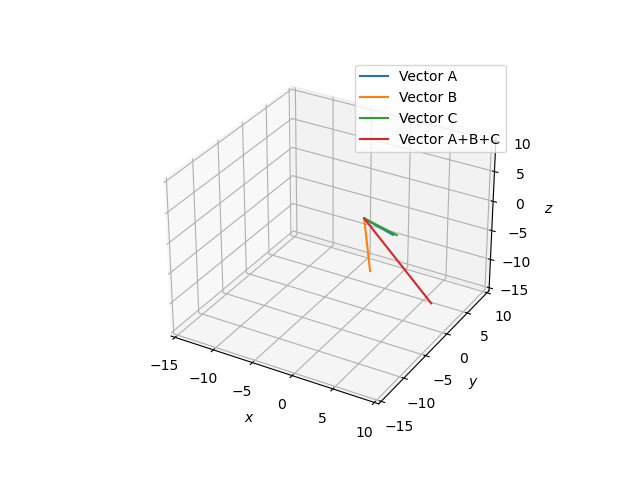
\includegraphics[width=\columnwidth, height=0.8\textheight, keepaspectratio]{../figs/fig.png}     
\end{frame}

\begin{frame}[fragile]
    \frametitle{C Code (0) - Importing libraries}

    \begin{lstlisting}
#include <stdio.h>
#include <stdlib.h>
#include <string.h>
#include <math.h>
#include <sys/socket.h>
#include <netinet/in.h>
#include <unistd.h>
#include "libs/matfun.h"
#include "libs/geofun.h"
    \end{lstlisting}
\end{frame}
\begin{frame}[fragile]
    \frametitle{C Code (1) - Function to Generate Points on a Line}

    \begin{lstlisting}

void point_gen(FILE *p_file, double **A, double **B, int rows, int cols, int npts){
    for(int i = 0; i <= npts; i++){
     double **output = Matadd(A, Matscale(Matsub(B, A, rows, cols), rows, cols, (double)i/npts), rows, cols);
     fprintf(p_file, "%lf, %lf, %lf\n", output[0][0], output[1][0], output[2][0]);
     freeMat(output, rows);
    }
}

    \end{lstlisting}
\end{frame}


\begin{frame}[fragile]
    \frametitle{C Code (2) - Function to write points b/w given point and origin to a file}

    \begin{lstlisting}
float find_norm(double **p, int n);

int write_points(double x1, double y1, double z1, double x2, double y2, double z2, double x3, double y3, double z3, int npts){
    int m = 3;
    int n = 1;

    double **R = createMat(m, n);
    double **O = createMat(m, n);
    double **T = createMat(m, n);
    double **S = createMat(m, n);
    double **origin = createMat(m, n);

    for(int i = 0; i<3; i++)
        origin[i][0] = 0; 
    

    \end{lstlisting}
\end{frame}
\begin{frame}[fragile]
    \frametitle{C Code (2) - Function to write points b/w given point and origin to a file}

    \begin{lstlisting}
    R[0][0] = x2;
    R[1][0] = y2;
    R[2][0] = z2;

    O[0][0] = x1;
    O[1][0] = y1;
    O[2][0] = z1;

    T[0][0] = x1+x2+x3;
    T[1][0] = y1+y2+y3;
    T[2][0] = z1+z2+z3;

    S[0][0] = x3;
    S[1][0] = y3;
    S[2][0] = z3;
    \end{lstlisting}
\end{frame}

\begin{frame}[fragile]
    \frametitle{C Code (2) - Function to write points b/w given point and origin to a file}

    \begin{lstlisting}
    FILE *p_file;
    p_file = fopen("plot.dat", "w");
    if(p_file == NULL)
        printf("Error opening one of the data files\n");
    point_gen(p_file, origin, O, m, n, npts);
    point_gen(p_file, origin, R, m, n, npts);
    point_gen(p_file, origin, S, m, n, npts);
    point_gen(p_file, origin, T, m, n, npts);
    float k = find_norm(T, m);
    freeMat(R, m);
    freeMat(O, m);
    freeMat(T, m);
    freeMat(S, m);
    freeMat(origin, m);
    fclose(p_file);
    return k;
    }
    \end{lstlisting}
\end{frame}


\begin{frame}[fragile]
    \frametitle{C Code (3) - Finding norm}

\begin{lstlisting}
float find_norm(double **p, int n){
    return sqrt(Matmul(transposeMat(p, n, 1), p, 1, n, 1)[0][0]);
}
\end{lstlisting}
\end{frame}

\begin{frame}[fragile]
    \frametitle{Python Code (0) - Importing libraries and checking system}
    \begin{lstlisting}
import numpy as np
import matplotlib.pyplot as plt
import ctypes
import os
import sys
import subprocess

print('Using termux? (y/n)')
termux = input()
\end{lstlisting}
\end{frame}

\begin{frame}[fragile]
    \frametitle{Python Code (1) - Using Shared Object}
    \begin{lstlisting}
lib_path = os.path.join(os.path.dirname(__file__), 'plot.so')
my_lib = ctypes.CDLL(lib_path)

my_lib.write_points.argtypes = [ctypes.c_double, ctypes.c_double, ctypes.c_double, ctypes.c_double, ctypes.c_double, ctypes.c_double, ctypes.c_double, ctypes.c_double, ctypes.c_double, ctypes.c_int]
my_lib.write_points.restype = ctypes.c_float
p1 = np.array([2, 3, -4])
p2 = np.array([3, -4 , -5])
p3 = np.array([3, 2, -3])
npts = 20000
k = my_lib.write_points(p1[0], p1[1], p1[2], p2[0], p2[1], p2[2], p3[0], p3[1], p3[2], npts)
\end{lstlisting}
\end{frame}

\begin{frame}[fragile]
    \frametitle{Python Code (2) - Loading points and finding norm}
    \begin{lstlisting}
print(f'The norm of A+B+C = {k}')

points = np.loadtxt('plot.dat', delimiter=',', usecols = (0,1, 2))[0:npts+1]
points2 = np.loadtxt('plot.dat', delimiter=',', usecols = (0,1, 2))[npts+1:2*(npts+1)]
points3 = np.loadtxt('plot.dat', delimiter =',', usecols = (0,1,2))[2*(npts+1):3*(npts+1)]
points4 = np.loadtxt('plot.dat', delimiter =',', usecols = (0,1,2))[3*(npts+1):4*(npts+1)]
\end{lstlisting}
\end{frame}

\begin{frame}[fragile]
    \frametitle{Python Code (2) - Loading points and finding norm}
    \begin{lstlisting}
        x = points[:, 0]
        y = points[:, 1]
        z = points[:, 2]
        
        x2 = points2[:, 0]
        y2 = points2[:, 1]
        z2 = points2[:, 2]
        
        x3 = points3[:, 0]
        y3 = points3[:, 1]
        z3 = points3[:, 2]
        
        x4 = points4[:, 0]
        y4 = points4[:, 1]
        z4 = points4[:, 2]
    \end{lstlisting}
\end{frame}

\begin{frame}[fragile]
    \frametitle{Python Code (3) - Plotting points}
    \begin{lstlisting}
fig = plt.figure()
ax = fig.add_subplot(111, projection = '3d')
ax.plot(x, y, z, label = 'Vector A')
ax.plot(x2, y2, z2, label = 'Vector B')
ax.plot(x3, y3, z3, label = 'Vector C')
ax.plot(x4, y4, z4, label = 'Vector A+B+C')

ax.set_xlabel('$x$')
ax.set_ylabel('$y$')
ax.set_zlabel('$z$')
ax.legend(loc='best')
ax.grid() 
ax.axis('equal')
ax.set_xlim([-15, 10])
ax.set_ylim([-15, 10])
ax.set_zlim([-15, 10])

\end{lstlisting}
\end{frame}

\begin{frame}[fragile]
    \frametitle{Python Code (4) - Saving plot and opening it}
    \begin{lstlisting}
fig.savefig('../figs/fig2.png')
print('Saved figure to ../figs/fig2.png')

if(termux == 'y'):
    subprocess.run(shlex.split('termux-open ../figs/fig2.png'))
else:
    subprocess.run(["open",  "../figs/fig2.png"])
\end{lstlisting}
\end{frame}

\begin{frame}{Plot-Using Both C and Python}
    \centering
    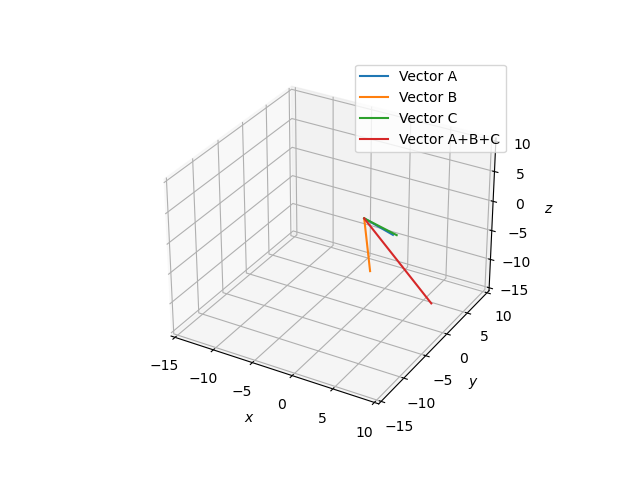
\includegraphics[width=\columnwidth, height=0.8\textheight, keepaspectratio]{../figs/fig2.png}     
\end{frame}

\end{document}